\documentclass[a4paper,12pt]{article}
\usepackage{../../mypackages}
\usepackage{../../macros}

\setlength{\parindent}{0pt}


\begin{document}

\title{Feuille d'exercices supplémentaires - L'atome}
\author{N. Bancel}
\date{4 Décembre 2024}
\maketitle

\section{Exercice 1}

En s'inspirant de l'exercice corrigé ci-dessous, résoudre l'exercice suivant portant sur les bruleurs au bioéthanol.

\begin{figure}[H]
  \centering
  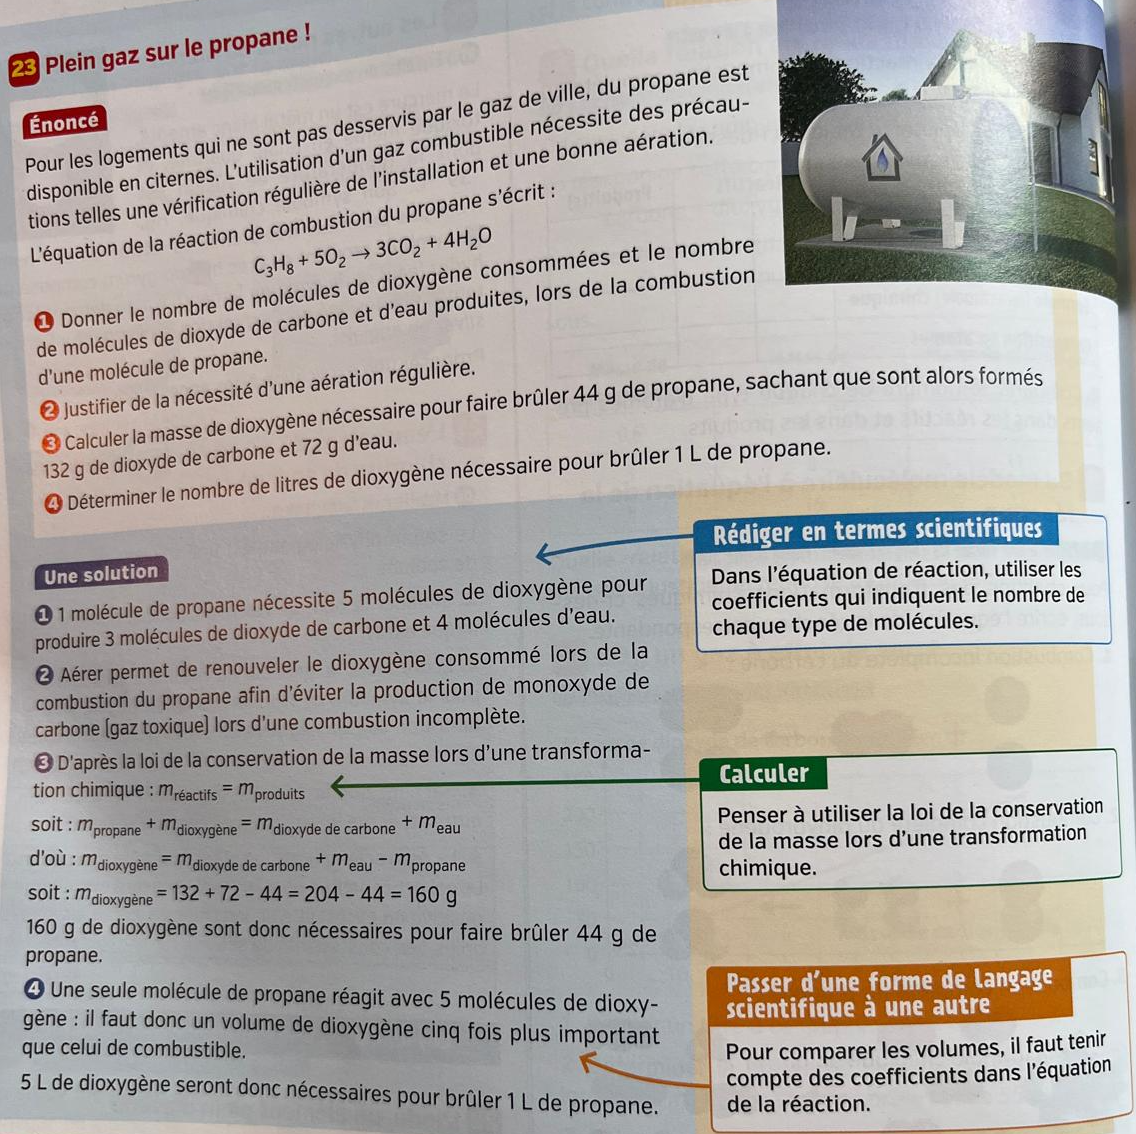
\includegraphics[width=0.8\linewidth]{img/04_03_01.png}
  \caption{\label{} Le propane}
\end{figure}

De nos jours, il existe des brûleurs au bioéthanol qui s'insèrent dans la cheminée. Le bioéthanol (alcool de betterave, constitué de molécules d'éthanol) remplace alors le bois comme combustible. L'équation de cette combusion s'écrit : 
\[
\ce{C2H6O + 3 O2 -> 2 CO2 + 3 H2O}
\]
\begin{itemize}[noitemsep]
  \item Donner le nombre de molécules de dioxygène consommées et le nombre de molécules de dioxyde de carbone et d'eau produites lors de la combustion d'une molécule d'éthanol.
  \item Calculer la masse de dioxygène nécessaire pour faire brûler 1180g d'éthanol sachant qu'il se forme 2257g de dioxyde de carbone et 1305g d'eau.
  \item Calculer le nombre de litres de dioxyde de carbone produits lorsque 6L de dioxygène sont consommés
\end{itemize}

\section{Exercice 2 - Le transport routier}

\begin{figure}[H]
  \centering
  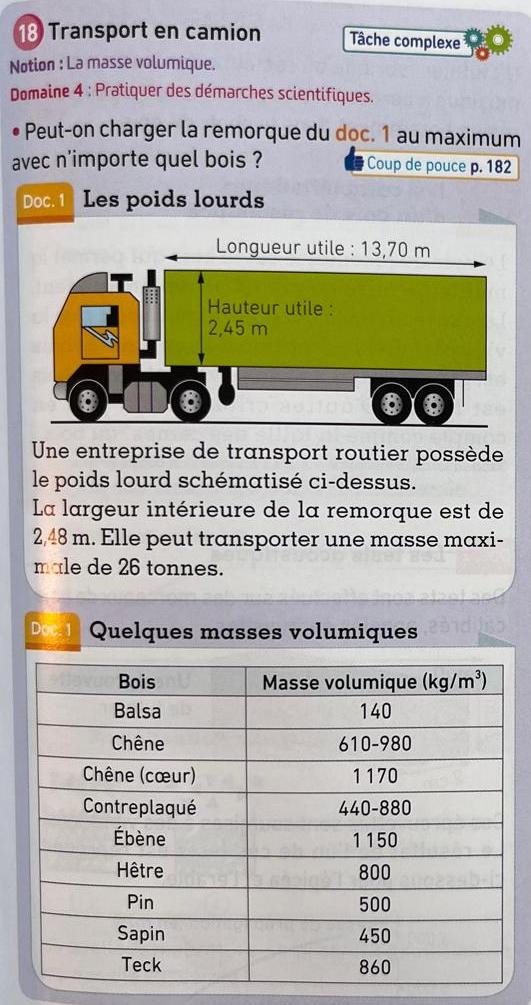
\includegraphics[width=0.3\linewidth]{img/04_03_02.jpeg}
  \caption{\label{} Exercice 3}
\end{figure}


\section{Exercice 3 - La pétanque}

\begin{figure}[H]
  \centering
  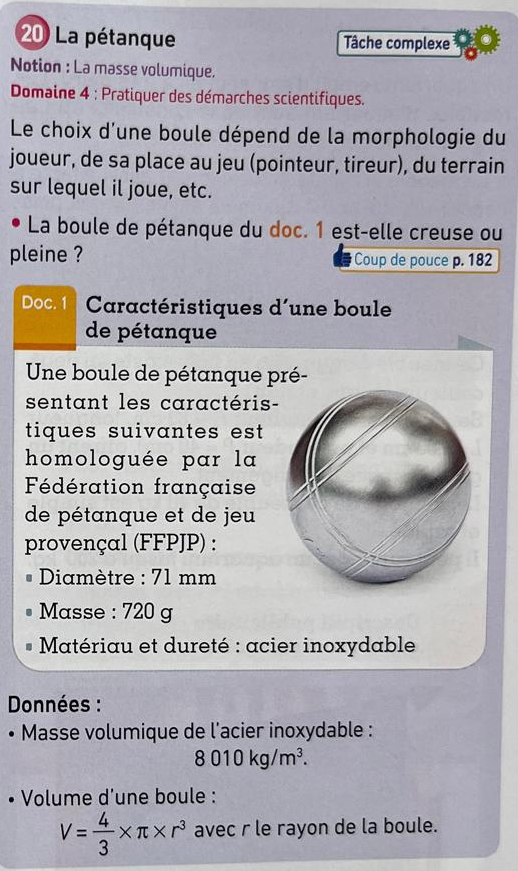
\includegraphics[width=0.3\linewidth]{img/04_03_03.png}
  \caption{\label{} Exercice 4}
\end{figure}

\section{Corrigé - Exercice 1}

L'équation de la combustion de l'éthanol est donnée :
\[
\ce{C2H6O + 3 O2 -> 2 CO2 + 3 H2O}
\]

\textbf{Tout d'abord on vérifie que l'équation est bien équilibrée}. Pour cela, il faut que la masse se conserve : c'est-à-dire qu'on doit retrouver le même type et le même nombre d'atomes de chaque type côté réactifs et côté produits. On va donc décompter :

\begin{itemize}
\item \textbf{Types et nombre d'atomes - Côté réactifs :}
  \begin{itemize}
    \item \textbf{Carbone (\ce{C}) :} Il y a 2 atomes de carbone dans la molécule \ce{C2H6O}. Donc, il y a au total 2 atomes de carbone côté réactifs.
    \item \textbf{Hydrogène (\ce{H}) :} Il y a 6 atomes d'hydrogène dans la molécule \ce{C2H6O}. Donc, il y a au total 6 atomes d'hydrogène côté réactifs.
    \item \textbf{Oxygène (\ce{O}) :} 
      \begin{itemize}
        \item La molécule \ce{C2H6O} contient 1 atome d'oxygène.
        \item Les 3 molécules de dioxygène \ce{3O2} contiennent chacune 2 atomes d'oxygène, soit \(3 \times 2 = 6\) atomes d'oxygène.
      \end{itemize}
      Au total, il y a \(1 + 6 = 7\) atomes d'oxygène côté réactifs.
  \end{itemize}

\item \textbf{Types et nombre d'atomes - Côté produits :}
  \begin{itemize}
    \item \textbf{Carbone (\ce{C}) :} Il y a 2 molécules de dioxyde de carbone \ce{CO2}, chacune contenant 1 atome de carbone. Donc, il y a \(2 \times 1 = 2\) atomes de carbone côté produits.
    \item \textbf{Hydrogène (\ce{H}) :} Il y a 3 molécules d'eau \ce{H2O}, chacune contenant 2 atomes d'hydrogène. Donc, il y a \(3 \times 2 = 6\) atomes d'hydrogène côté produits.
    \item \textbf{Oxygène (\ce{O}) :} 
      \begin{itemize}
        \item Les 2 molécules de dioxyde de carbone \ce{CO2} contiennent chacune 2 atomes d'oxygène, soit \(2 \times 2 = 4\) atomes d'oxygène.
        \item Les 3 molécules d'eau \ce{H2O} contiennent chacune 1 atome d'oxygène, soit \(3 \times 1 = 3\) atomes d'oxygène.
      \end{itemize}
      Au total, il y a \(4 + 3 = 7\) atomes d'oxygène côté produits.
  \end{itemize}
\end{itemize}

\textbf{Conclusion :} On constate que :
\begin{itemize}
  \item Le nombre d'atomes de carbone est identique : \(2 = 2\),
  \item Le nombre d'atomes d'hydrogène est identique : \(6 = 6\),
  \item Le nombre d'atomes d'oxygène est identique : \(7 = 7\).
\end{itemize}

Ainsi, l'équation est bien équilibrée.


Cette équation montre les proportions stœchiométriques entre les réactifs et les produits :
\begin{itemize}
\item 1 molécule d'éthanol (\ce{C2H6O}) réagit avec 3 molécules de dioxygène (\ce{O2}),
\item et produit 2 molécules de dioxyde de carbone (\ce{CO2}) et 3 molécules d'eau (\ce{H2O}).
\end{itemize}

Autrement dit : Lors de la combustion d'une molécule d'éthanol :
\begin{itemize}
    \item \textbf{Nombre de molécules de \ce{O2} consommées :} 3 molécules,
    \item \textbf{Nombre de molécules de \ce{CO2} produites :} 2 molécules,
    \item \textbf{Nombre de molécules de \ce{H2O} produites :} 3 molécules.
\end{itemize}

\subsection*{2. Masse de dioxygène nécessaire pour brûler 1180 g d'éthanol}

On sait que la masse se conserve lors d'une réaction chimique. Donc $m_réactifs = m_produits$. Autrement dit : 

\[
m_{bioéthanol} + m_{dioxygène} = m_{dioxyde\_carbone} + m_{eau}
\] 

\[
m_{dioxygène} = m_{dioxyde\_carbone} + m_{eau} - m_{bioéthanol}
\] 

\vspace{1em}
\textbf{Application numérique}
\vspace{1em}

$m_{dioxyde\_carbone} = \SI{2257}{g}$ \\
$m_{eau} = \SI{1305}{g}$ \\
$m_{bioéthanol} = \SI{1180}{g}$ \\

Donc : 

\[
m_{dioxygène} = 2257 + 1305 - 1180
\] 

\[
m_{dioxygène} = 2382 \si{g}
\] 

\subsection*{3. Volume de \ce{CO2} produit lorsque 6 L de \ce{O2} sont consommés}

\subsubsection*{Étape 1 : Relation entre les volumes dans les gaz parfaits}
Dans les mêmes conditions de température et de pression, les volumes des gaz sont proportionnels à la quantité de matière qui réagit ou qui est produite. D'après l'équation chimique, 3 volumes de \ce{O2} donnent 2 volumes de \ce{CO2}. On peut résumer cela sous la forme d'un tableau : 

\vspace{1em}
\begin{center}
\begin{tabular}{SS}
  \toprule
  {$V_{\ce{O2}}$} & {$V_{\ce{CO2}}$} \\
  \midrule
  {3} & {2} \\
  \bottomrule
\end{tabular}
\end{center}

\vspace{1em}

Avec un produit en croix, on peut dire que 

\[
3 \times V(\ce{CO2}) = 2 \times V(\ce{O2})
\]

c'est-à-dire 

\[
V(\ce{CO2}) = \frac{2}{3} \times V(\ce{O2})
\]

\subsubsection*{Étape 2 : Calcul du volume de \ce{CO2} produit}
Si 6 L de \ce{O2} sont consommés :
\[
V(\ce{CO2}) = \frac{2}{3} \times V(\ce{O2})
\]
\[
V(\ce{CO2}) = \frac{2}{3} \times 6 = 4 \, \si{\liter}
\]

\textbf{Réponse explicite :} Le volume de dioxyde de carbone produit est \(\mathbf{4 \, \si{\liter}}\).

\section{Corrigé - Exercice 2 - Transport routier}

\subsection*{Résolution}
\paragraph{Étape 1 : Calcul du volume de la remorque}
Le volume utile de la remorque est donné par :
\[
V = \text{longueur} \times \text{largeur} \times \text{hauteur}
\]
\[
V = 13,70~\text{m} \times 2,48~\text{m} \times 2,45~\text{m} = 82,9732~\text{m}^3
\]

\paragraph{Étape 2 : Masse totale possible pour chaque bois}
La masse totale d'un bois remplissant entièrement la remorque est donnée par :
\[
m = \rho \times V
\]
où $\rho$ est la masse volumique du bois (en $\text{kg/m}^3$).

Pour chaque bois, on calcule les masses maximales correspondantes :
\[
\text{Balsa} : m = 140 \times 82,9732 \approx 11~616~\text{kg}
\]
\[
\text{Chêne (min)} : m = 610 \times 82,9732 \approx 50~614~\text{kg}
\]
\[
\text{Chêne (max)} : m = 980 \times 82,9732 \approx 81~314~\text{kg}
\]
\[
\text{Chêne (cœur)} : m = 1~170 \times 82,9732 \approx 97~076~\text{kg}
\]
\[
\text{Contreplaqué (min)} : m = 440 \times 82,9732 \approx 36~508~\text{kg}
\]
\[
\text{Contreplaqué (max)} : m = 880 \times 82,9732 \approx 72~891~\text{kg}
\]
\[
\text{Ébène} : m = 1~150 \times 82,9732 \approx 95~419~\text{kg}
\]
\[
\text{Hêtre} : m = 800 \times 82,9732 \approx 66~379~\text{kg}
\]
\[
\text{Pin} : m = 500 \times 82,9732 \approx 41~487~\text{kg}
\]
\[
\text{Sapin} : m = 450 \times 82,9732 \approx 37~339~\text{kg}
\]
\[
\text{Teck} : m = 860 \times 82,9732 \approx 71~357~\text{kg}
\]

\paragraph{Étape 3 : Comparaison avec la masse maximale transportable}
La remorque peut transporter une masse maximale de $26~000~\text{kg}$. En comparant les masses calculées :
\begin{itemize}
    \item Seul le balsa peut être chargé au maximum ($m \approx 11~616~\text{kg} < 26~000~\text{kg}$).
    \item Tous les autres bois dépassent cette limite et ne peuvent pas remplir complètement la remorque.
\end{itemize}

\subsection*{Conclusion}
Il est possible de charger la remorque au maximum uniquement avec du balsa. Les autres types de bois, à cause de leur masse volumique élevée, dépassent la masse maximale autorisée pour le camion.


\section*{Correction : La boule de pétanque est-elle creuse ou pleine ?}

\subsection*{Problème posé}
On cherche à déterminer si la boule de pétanque est creuse ou pleine, en comparant sa masse réelle à la masse théorique calculée pour une boule pleine.

\subsection*{Données}
\begin{itemize}
    \item Masse de la boule : $m = 720~\text{g} = 0,720~\text{kg}$.
    \item Diamètre de la boule : $d = 71~\text{mm} = 0,071~\text{m}$.
    \item Masse volumique de l'acier inoxydable : $\rho = 8~010~\text{kg/m}^3$.
    \item Formule du volume d'une boule :
    \[
    V = \frac{4}{3} \pi r^3 \quad \text{avec } r \text{ le rayon de la boule.}
    \]
\end{itemize}

\subsection*{Résolution}
\paragraph{Étape 1 : Calcul du volume de la boule}
Le rayon de la boule est :
\[
r = \frac{d}{2} = \frac{0,071}{2} = 0,0355~\text{m}.
\]

Le volume de la boule est alors donné par :
\[
V = \frac{4}{3} \pi r^3 = \frac{4}{3} \pi (0,0355)^3.
\]

Effectuons les calculs :
\[
V = \frac{4}{3} \pi \times 0,0000447 \approx 0,0001875~\text{m}^3.
\]

\paragraph{Étape 2 : Calcul de la masse théorique pour une boule pleine}
La masse théorique d'une boule pleine est donnée par :
\[
m_{\text{pleine}} = \rho \times V.
\]

Substituons les valeurs :
\[
m_{\text{pleine}} = 8~010 \times 0,0001875 \approx 1,501~\text{kg}.
\]

\paragraph{Étape 3 : Comparaison avec la masse réelle}
La masse réelle de la boule est de $0,720~\text{kg}$. Cette masse est bien inférieure à la masse théorique pour une boule pleine ($1,501~\text{kg}$).

\subsection*{Conclusion}
La boule de pétanque est creuse. Si elle était pleine, sa masse serait beaucoup plus élevée.



\end{document}
